\chapter{Evaluation of Distributed MCTS Algorithms}
\label{chap_evaluation}

\section{Ms Pac-Man vs Ghosts Framework}
\label{sec_pacman_vs_ghosts}

For the purposes of evaluation of algorithms proposed in Chapter \ref{chap_dmcts_design}, we
have chosen the Ms Pac-Man vs Ghosts Framework \cite{PacmanVsGhosts} which is easy-to-use
framework allowing implementation of players for well-known old game Pac-Man in Java. Here we
will extract basics of the game rules used in the framework and afterwards we will
describe modifications of the rules we have done and reasons for them.

\subsection{Game Rules}

Ms Pac-Man is a game played in a maze in which two sides compete, the Pac-Man and four ghosts.
There are pills everywhere in the maze and Pac-Mans purpuse is to gather all the pills, each
for 10 points. Once all the pills are eaten, the game continues in a next maze. To complicate
the life of Pac-Man, ghosts are moving around the maze pursuing the Pac-Man and trying to
minimize its score. If the Pac-Man is caught, it will lose one life and if has any life
remaining, starts again from its starting position. Pills remain eaten after the life loss.
Ghosts appear in so-called lair at the beginning of each round and after Pac-Man's life loss
from where they start after a several time (different for each ghost). Beside regular pills,
each maze contains four power pills which are awarded with 50 points and when eaten by Pac-Man,
ghosts become edible and twice slower for certain period of time. Pac-Man can eat ghosts during 
this period for
reward of 200 points for first eaten ghost and 400, 800 and 1600 points for other ghosts.
Eaten ghost starts in lair again. Exact rules of the Ms Pac-Man vs Ghosts game can be found on the project webpage. 

The game was
additionally modified for purposes of testing of our algorithms. Biggest change of rules is
removing power pills from the mazes together with entire edible ghosts mechanism. Reason for
this decision is lowering the variability of results. When Pac-Man is pursuing edible ghosts,
there is big difference in score when it eats different number of ghosts. For the same reason
three more modifications have been done. Pac-Man has only one life, game ends after the first
maze is cleared and random ghosts' reversal is suppressed. Random ghosts' reversal is a rule of
original Ms Pac-Man game bringing stochasticity to the game. If the rule is on, there is a 0.15\% 
probability each tick of a game that all
ghosts accidentally change their direction. Original game has a limit on maximum length of each
round after which score for remaining pills is added to Pac-Man's score and game continues to
the next level. This limit is set to 2000 what we keep as a rule, so our simplified game ends
after at most 2000 ticks. Limiting the number of rounds played together with limit on game
length also lets us run more tests.
An example of a situation from the game without
power pills is depicted by Figure \ref{fig_pacman_framework}.

\begin{figure}
\begin{center}
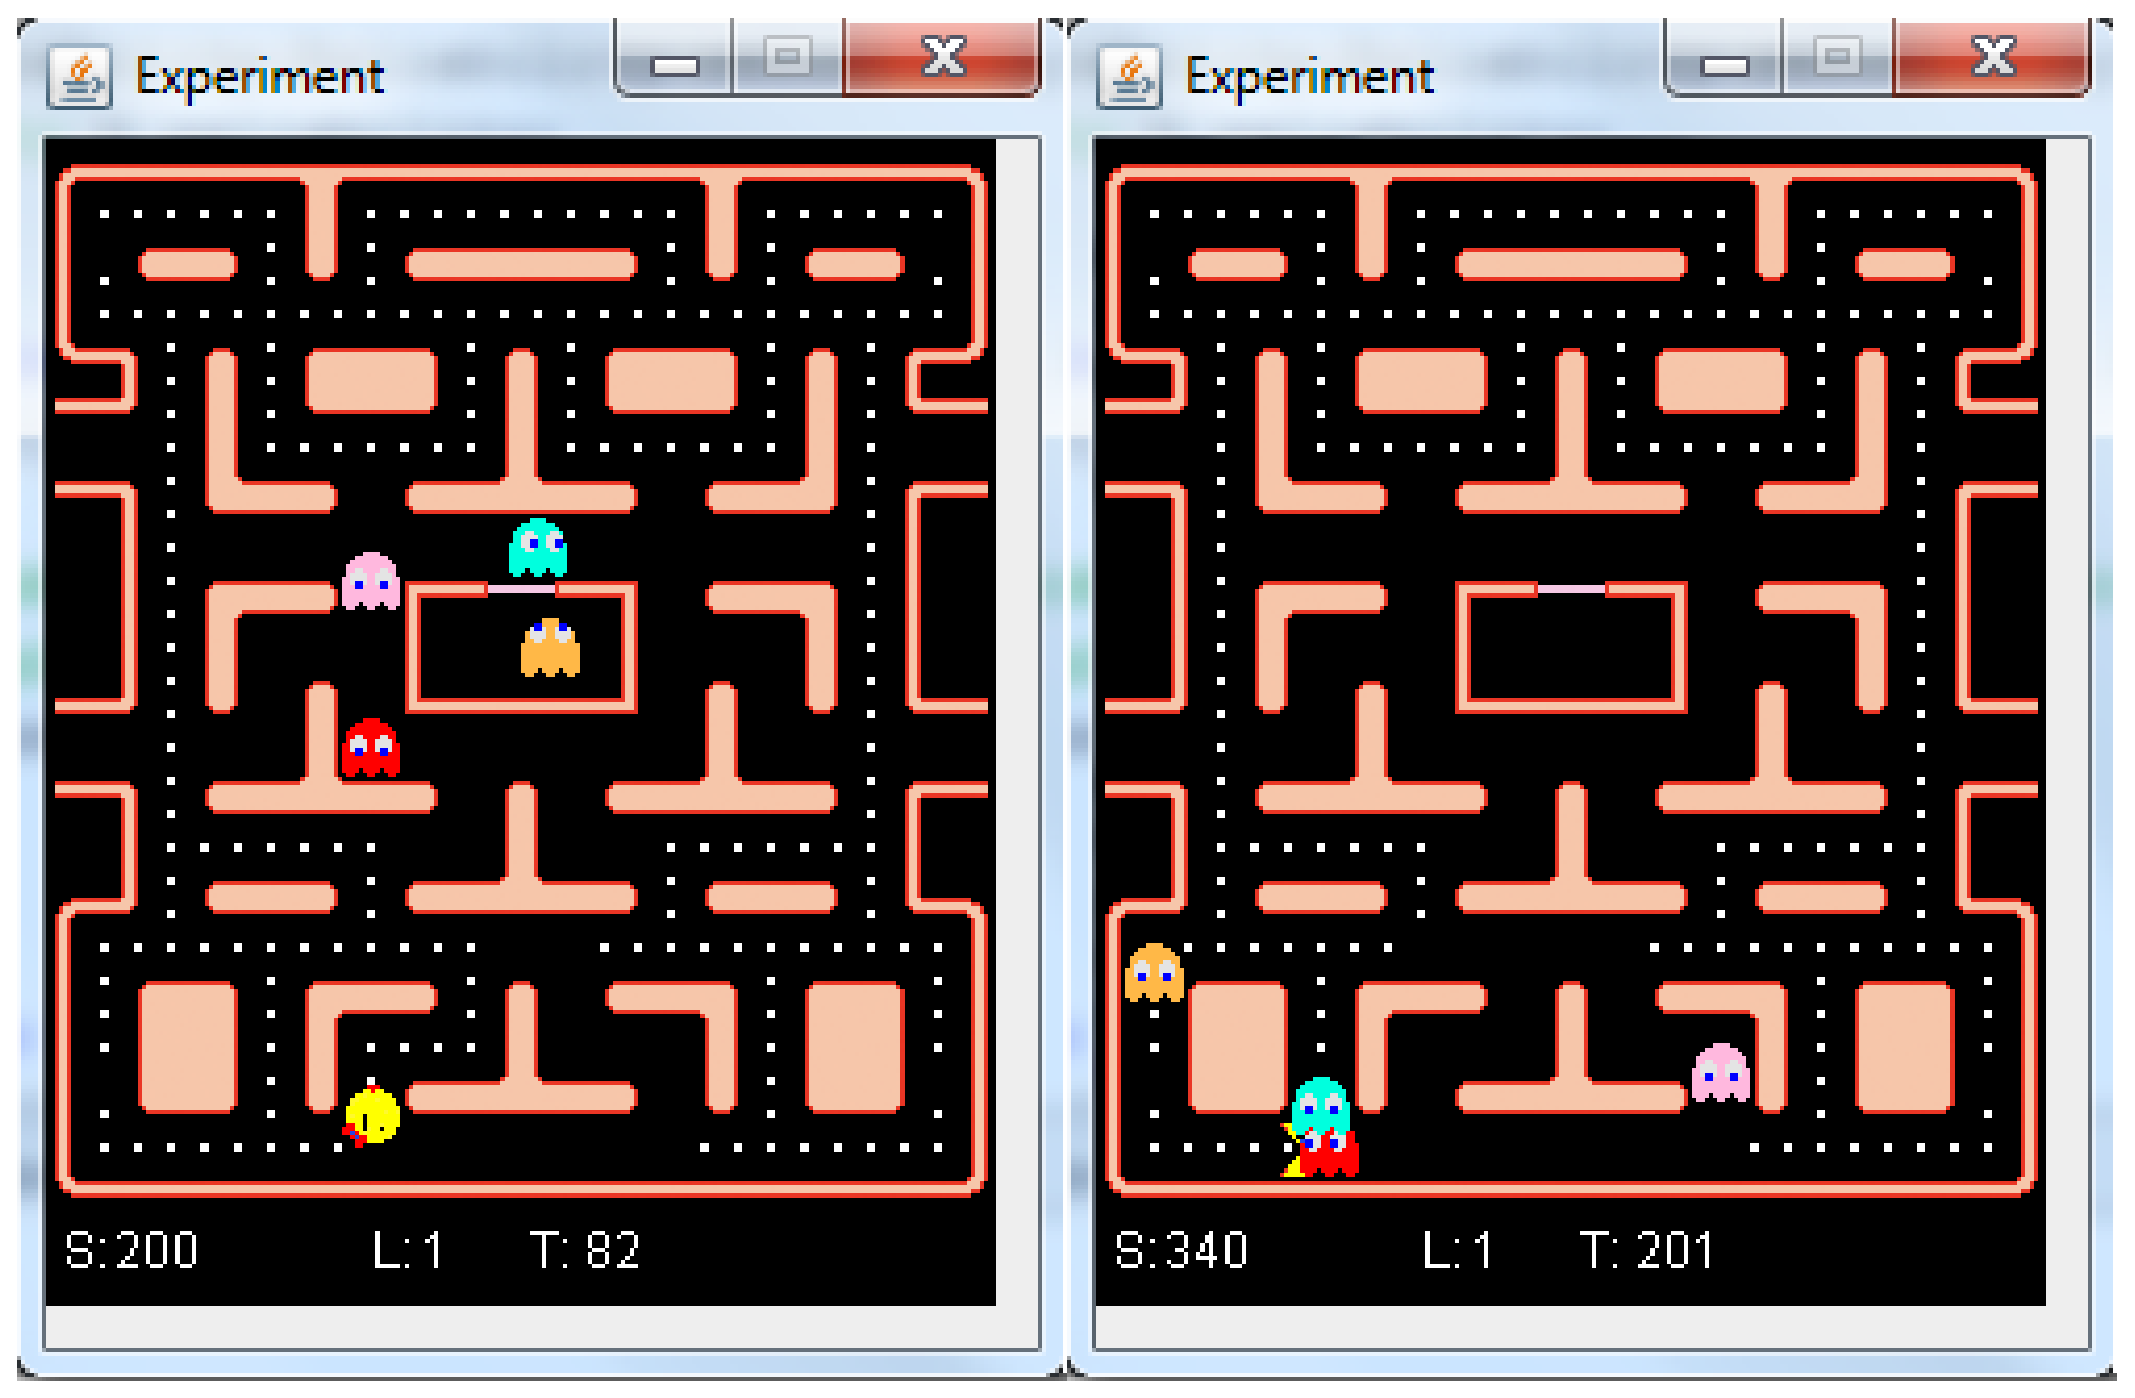
\includegraphics[width=14cm]{img/pacman_framework.eps}
\end{center}
\caption{\footnotesize Simplified game of Ms Pacman.}{\footnotesize Left picture shows the game few moments after it began. Three
ghosts started to hunt the Pac-Man while the orange one is still waiting in lair. Right
picture, on the other hand, shows the game just before the end. Pac-Man does not have any
escape path and is being caught with in a while with no life remaining.}
\label{fig_pacman_framework}
\end{figure}

Pac-Man has the same movement speed as non-edible ghosts. Paths inside the maze are divided
into small segments, four between two neighbouring pills. Pac-Man has to play an action after
at each segment, turning back in the middle of path or at the crossroad is allowed and so
Pac-Man has always at least two action to choose between. Contrarily, ghosts' movement is
restricted. Additional rule on ghosts' movement is that ghosts cannot turn back in the middle
of a path nor at a crossroad. That means that once a ghost chooses one way from a crossroad, it
has to continue to the end of the path. Despite of that, ghosts have to play an action on each
segment even though there is only one action to choose from.

\todo{Porovnat Pac-Mana s pursuit-evasion game}

So Pac-Man and ghosts play their actions at each segment of the maze but they, of course, have
to play an action in a limited time. Ms Pac-Man vs Ghosts framework provides by default 40 ms
to play what corresponds with the natural game timing when a human player controls Pac-Man.


\subsection{Framework Details}

In our thesis, we use Ms Ghost vs Pacman framework version 6.2. The framework is written in
Java what simplifies the development of controllers of the players. In original game, player
was able to control only Pac-Man and ghosts were controlled by simple AI. In the framework,
it is also possible to develop controller for the ghosts. The only work a user is supposed to 
do is
implement a controller of Pac-Man or ghosts, methods for running a game or a set of games are
prepared for usage. 

A player controller is a class implementing an interface having only one
method. In case of ghosts controller, method's header is \texttt{public EnumMap<GHOST,MOVE>
getMove(Game game,long timeDue)}, where \texttt{EnumMap<GHOST,MOVE>} is a joint-action of
ghosts, \texttt{game} contains information of current game and \texttt{timeDue} contains time
until which the method has to return an action.
If an action is not returned on time, certain
default action is chosen by framework itself.



\subsection{Pac-Man Opponents and Simple Ghosts Controllers}

To evaluate the strength of ghost controllers based on distributed MCTS algorithms, we need to
choose appropriate Pac-Man opponent to play against. Unfortunately, experiments with Pac-Man
controllers included in Ms Pacman vs Ghosts framework showed that these controllers are too
weak for evaluation. Thus, it was necessary to look for better Pac-Man controllers. 

Main purpose of the Ms Pacman vs Ghosts project is organizing competitions between existing
controllers. Competitions are usually held on various conferences and meanwhile there is also a
league  in which all controllers commited into the website compete. Thanks to the leagure
results we were able to contact authors of the league leading Pac-Man and obtained source code
of ICEP\_IDDFS \cite{IcepIddfs} what is controller based on iterative deepening depth-first
search approach. We haven't received more details about the controller. However, experiments
running against it give promising results and so the controller was chosen as an opponent to
compare with.

\todo{Porovnat výkonnost starter controllerů}



\section{Implementation Notes}
\label{sec_implementation_notes}

In this section, we will discuss important implementation details of our controllers. As
mentioned in previous section, framework used for the experiments is written in Java and so
controllers are also supposed to be written in this language.


\subsection{Tree Construction}

Here we will talk about the way the concrete realization of MCTS tree for the game of Ms
Pac-Man. The most direct approach to a construction is to keep a node of the tree for each game
step and store, besides the value and the visit count, actions performed by Pac-Man and all
ghosts. By exposing and resolving of problems of this solution, we have reached the
construction used in our controllers.

First problem to be solved is that MCTS tree should not work with simultaneous actions of
multiple teams as discussed in Section \ref{sec_two_players_mcts}. 
Ms Pac-Man satisfies the definition of simultaneous game with teams, since multiple ghosts
together with Pac-Man may be on turn at a same time.
Section 
\ref{sec_turn_based_game_conversion} gives us a recipe to deal with simultaneous actions by
convertion of a simultaneous game to a (weak) turn-based game by splitting simultaneous nodes. The
conversion is not done on the unterlying Ms Pac-Man game itself but only for purposes of
expansion of nodes. When a simultaneous node is being expanded, instead of creating of a child
node for each pacman-ghosts joint-action, only children for each pacman action is created and
each of this children is immediately expanded with ghosts actions. By this approach,
simultaneous nodes are splitted accordingly to optimistic expansion since in such a tree the
ghosts suppose to know the action of Pac-Man played in the simultaneous node. Our
implementation, in addition, supports the pesimistic expansion where ghosts actions are
expanded first in simultaneous nodes.

Second problem is quite high branching factor caused by Pac-Man which is able to change its
direction at any time. To reduce the branching factor, we consider additional rules of Pac-Man's
movement for purposes of node expansion. We allow Pac-Man to change its direction only at
crossroads, in the neighbourhood of a segment with not yet eaten power pill and at segments in
the middle of path when last segment allowing the direction change is exactly 6 segments far.
When computing the MCTS tree for Pac-Man, this reduction does not bring any difficulty since
the player controlled by the algorithm follows additional rules. But if we consider Pac-Man
playing against the MCTS algorithm, it may play an action not corresponding with these rules what
directly leads to desynchronization between game state and built tree. Next time any ghost
reaches  a crossroad and the desynchronization is detected, ghost play an action accordingly to
the tree but then instead of using a subtree defined by the action for further computations,
new tree is built from scratch.

Finally, after expansion of simultaneous nodes and reduction of Pac-Man actions, the tree
will contain nodes having only one child which are also removed what adds a necessity to keep
lengths of edges between nodes.


\subsection{Pac-Man Playout}
\label{sec_impl_playout}

In our work, we decided to keep the simulation strategy simple, not leveraging much of
domain-specific information. This decision is driven by experiments from early phases of
development. During this experiments, both Pac-Man and ghosts players were, with a certain
probability, led by some heuristic algorithm inspired by original legacy behaviour in case of
ghost player and the StarterPacman example controller which is provided as a part of framework.
With supplementary probability, players performed random actions. Because we haven't discovered
any significant strength gain by tuning of the probability of heuristic steps, we omitted
heuristics at all.

The only additional knowledge put into the simulation strategy is that Pac-Man is not allowed
to change its direction in the middle of a path during simulation. The point of this 
restriction is that once Pac-Man enters a path, it usually wants to continue to a next
crossroad. In addition, such a restriction heightens expected size of area visited by Pac-Man
because situations of Pac-Man idling in the middle of path are suppressed.

We also use maximum depth of simulations. Tuning of this parameter is described in Section
\ref{sec_mcts_tuning}.

Simulations have to be evaluated after they finish. At first, we decided to use following
simple formula:

\begin{equation}
    { score\;reached } \over { maximum\;reachable\;score }
\end{equation}

But after some experiments, we realized that the formula does not enough motivate ghosts to
hunt pacman so we decided to add a bonus if ghosts successfully catch Pac-Man:

\begin{equation}
    (1 - \alpha) {{ score\;reached } \over { maximum\;reachable\;score }}
        + \alpha 
    \left\{
        \begin{array}{c@{\quad\quad}l}
            1 & if pacman\;was\;eaten\\
            0 & otherwise\\
        \end{array}
    \right.
\end{equation}

We call an $\alpha$ coefficient \emph{death\_weight} and tune it in Section
\ref{sec_mcts_tuning}.


\subsection{Communication}

Main method of a player controller (\texttt{getMove}) returns the joint-action
(\texttt{EnumMap<GHOST,MOVE>}) of the ghosts
but for purposes of distributed approach, each ghost is supposed to reason individually 
returning its action. To fulfil this, four subcontrollers, returning single \texttt{MOVE}
actions are started in four separated threads and virtual bidirectional communication 
channels are created between each pair of subcontrollers.

Channels provide interfaces for both senders and receivers and work with real time. Channel
consists of queue of messages to be sent and queue of received messages. Messages from the
sending queue to the receiving queue are transmitted every time a method on a channel is
called. Amount of messages transmitted corresponds with time elapsed since last channel event
ending with nonempty sending queue.

For purposes of evaluation of robustness of distributed algorithms againts communication
failures, channels contain a reliability object which simulates a reliability of a channel.
After a transmission of each message, the object determine if the message is really transmitted
to the receiver or if a failure occured and the message has to be discarded. The aim of the
reliability object is to filter messages to reach a percentual amount of messages successfully
transmitted. For the simplicity, we don't consider length of messages, messages of various
length have same probability of transmission. To model the reliability object closer to real
world, we decided not to use simple approach of single probability of transmission. Instead of
that, we work with two states of the object, \emph{reliable} and \emph{unreliable}, each
having a probability of successful transmission and a probability of a state change. In
reliable state, most of messages are transmitted and, contrariwise, most of messages are thrown
away in unreliable state. Such an
object is modelled as simple hidden Markov model depicted by Figure \ref{fig_hmm_reliability}.

\begin{figure}
\begin{center}
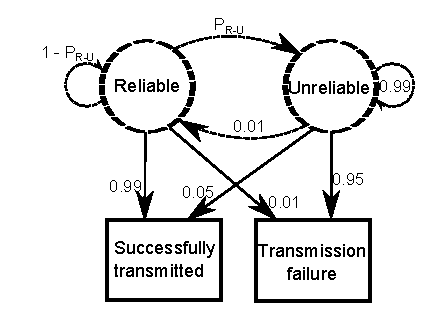
\includegraphics[width=8cm]{img/hmm_reliability.eps}
\end{center}
\caption{\footnotesize Communication reliability object modelled using hidden Markov model
used in our experiments.}{\footnotesize}
\label{fig_hmm_reliability}
\end{figure}

We permanently set three parameters of a model - probability of transmission in reliable and
unreliable state and probability of transition from unreliable to reliable model, denoted as
$P_{R}$, $P_{U}$ and $P_{U\mhyphen R}$. Remaining
parameter, a probability of transmission from reliable to unreliable state, denoted as
$P_{R \mhyphen U}$, is calculated accordinly to desired percentage of time in reliable state
$Rel$.
Transittion between states is done every millisecond. Then expected length of a single period
of the object remaining in unreliable state is $\mathrm{E}P_U = {1 \over P_{U\mhyphen R}} \times 1
\mathrm{ms} = {1
\over 0.01}\,\mathrm{ms} = 100\,\mathrm{ms}$. Expected length of a reliable-state period is
$\mathrm{E}P_R = {1 \over
P_{R\mhyphen U}}$. $Rel$ is then equal to $\mathrm{E}P_R \over \mathrm{E}P_R + \mathrm{E}P_U$ and so 
$P_{R\mhyphen U}$ is
calculated from $Rel$ by the following equation.

\begin{equation}
P_{R\mhyphen U} = { 1 - Rel \over Rel } P_{R\mhyphen U}
\end{equation}

In case of tests not considering a reliability, all messages are transmitted. For tests with
altering reliability, $Rel$ is set to value between $0$ and $1$ and appropriate $P_{R\mhyphen
U}$ is used in HMM model.



\section{Methodics}
\label{sec_methodics}

All experiments were performed in virtualized environment of CentOS release 6.3 (Final) having
assigned 12 CPUs and 16 GiB of memory. Underlying host server disposes of 2 Intel(R) Xeon(R) 
CPU E5-2630 0 @ 2.30GHz processors (6 cores/12 threads each) and total of 128 GiB of memory.
Beside of our testing server, a few other virtual servers were running on the host server with
a light consumption of resources but taking into account that we were leveraging at most 4
cores at a time, remaining cores could easily handle the traffic. 


Java runtime used for experiments is \texttt{1.7.0\_09-icedtea}.

Simple bash scripts were used for purpuses of launching of individual games. Our Java
application contains uniform entry point allowing setting of necessary parameters for running
of an experiment. Each experiment were performed 100 times and average values were then used.
Data gathered during experiments were then processed in R environment. Graphs contained in this
work are also generated with R.


\section{MCTS Tuning}
\label{sec_mcts_tuning}

\begin{figure}
\begin{center}
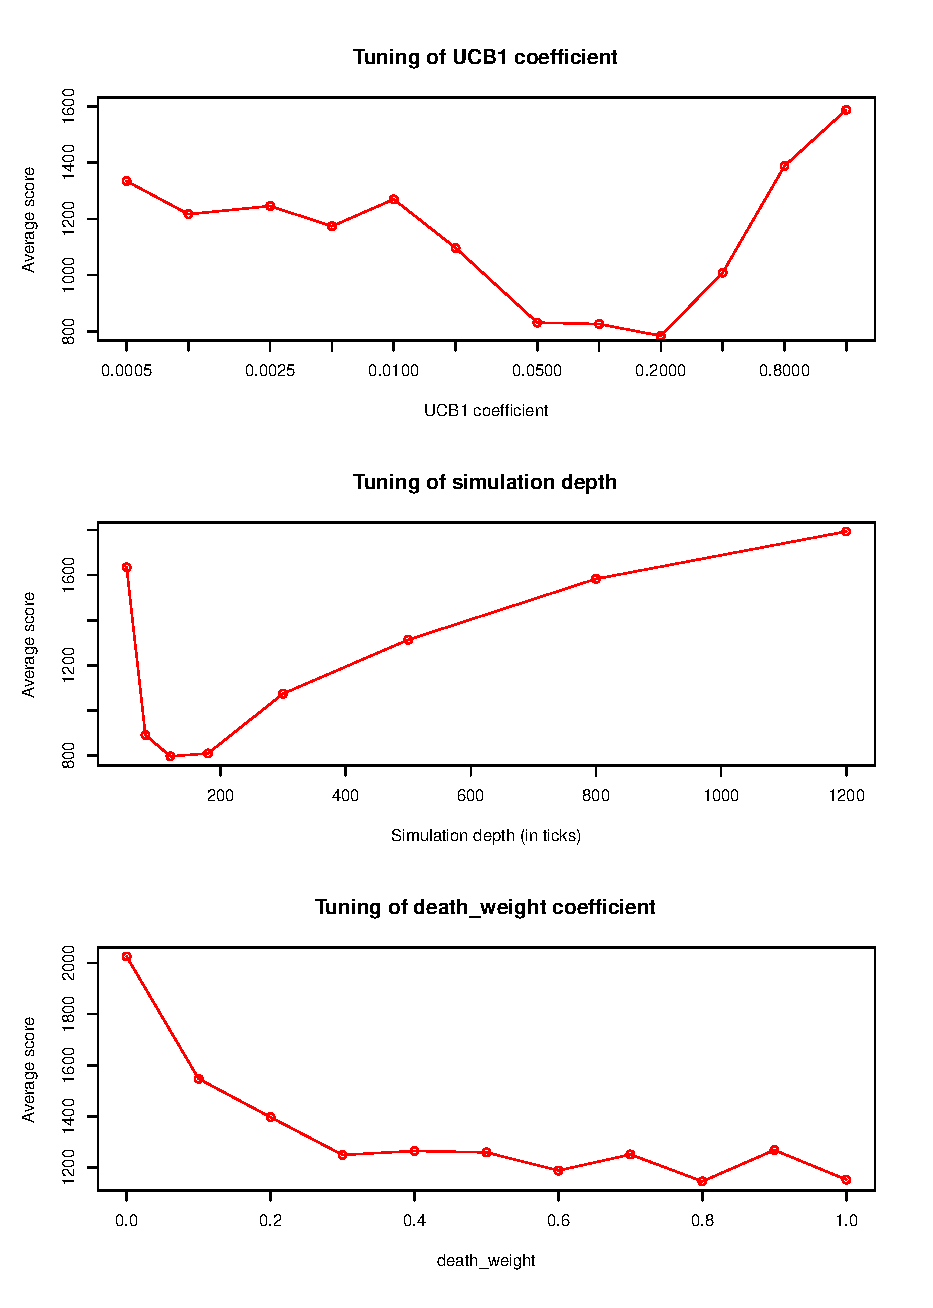
\includegraphics{img/mcts-tuning.eps}
\end{center}
\caption{\footnotesize Lorem ipsum}{\footnotesize }
\label{fig_mcts_tuning}
\end{figure}

Before we started any of our experiments, we wanted to be sure that our MCT alrogithm has
appropriate setting of parameters. We did three tests for approximate tuning of three
parameters - $C$ (UCT coefficient), simulation depth and \emph{death\_weight} (parameter used in
evaluation function, see Section \ref{sec_impl_playout}). Graphical results of these tests are
depicted by Figure \ref{fig_mcts_tuning}. All tunings were performed with a time ticks of 40
ms.

We first tuned $C$, with initial setting of simulation depth 200 and death weight 0.25. Test
showed us significant improvements with $C$ between 0.05 and 0.2 so we decided to use $C=0.1$.

Secondly, we tuned maximum depth of simulations, with already tuned $C=0.1$ and initial
$death\_weight=0.25$. Accordingly to the test, we set simulation depth to 120.

Finally, we tuned $death\_weight$ parameter used in evaluation formula with already tuned MCTS
parameters $C$ and simulation depth. Accordingly to the test, best values of the parameter are
between 0.3 and 1.0. During the evaluation of the test, some experiments with
$death\_weight=0.25$ were performing and a score with this $death\_weight$ didn't differ much,
we decided not to repeat the experiment with better setting of the parameter and run all tests
with $death\_weight=0.25$.



\section{Comparison of the Algorithms}
\label{sec_dmcts_experiments_comparison}

\todo{Okomentovat hodnoty simulations-per-second}

For distributed MCTS, three basic tests were performed. At first, strength of an algorithm
depending on computational time (length of single tick) with times from 10 ms to 200 ms, 100\%
reliable channel and channel speed fixed to a value of expected optimal communication
requirements. Second
test was strength in dependence on channel speed with fixed time set to 40 ms. Range of speeds
used depends on expected requirements on the communication so values
vary between tests. Channel speeds are scaled exponentially with values from $2^{lb}$ to
$2^{ub}$ for some algorithm-dependent values $lb,ub \in \mathbb{R}$.

We recall that the aim of the ghosts is minimization of Pac-Man's score so lesser score indicates
better performance of the ghosts.

Next to the final score, we measured various other characteristics, such as average number of simulations
performed per second, average size of MCTS tree at moments requiring a decision or real ammount
of communication. These characteristics simplified analysis of behaviour of the algorithms.


\subsection{Centralized Monte-Carlo Tree Search}


\begin{figure}
\begin{center}
\includegraphics[width=12cm]{img/plain-mcts-strength.eps}
\end{center}
\caption{\footnotesize Lorem ipsum}{\footnotesize }
\label{fig_plain_mcts_strength}
\end{figure}


In Section \ref{sec_measures_distributed}, we defined the strength-speedup measure which
is used for comparison of distributed algorithms with plain (centralized) algorithm. So 
before we perform experiments with distributed algorithm, we run experiments with plain MCTS.
During these tests, we also compare approaches to expansion of simultaneous nodes in Ms Pac-Man
game. Average number of simulations calculated per second by plain MCTS algorithm was 11002.
This number will be also used for comparison of algorithm.

Figure \ref{fig_plain_mcts_strength} depicts results of plain MCTS running on single processor.
We tested both optimistic and pesimistic expansion of simultaneous nodes. Since results didn't 
show a difference in performance of MCTS using these expansion, we have chosen, without
additional reasoning, a pesimistic expansion for further experiments.

A shape of the curve connecting measured points in the figure does not follow decreasing
progression which is, of course, caused by measurement error and local minima overcame by the
convergence of MCTS. However, for purposes of the strength-speedup measure, we need to have
smooth and decreasing function of strength of plain MCTS. For the sake of the measure, we
calculate such a function by polynomial regression. We fitted measured data of plain MCTS with
pesimistic expansion on polynomial function $S(t) = c_0 + { c_1 \over \sqrt{t} }$, where $S$ stands
for strength (or score), $c_0,c_1$ are fitted
coefficients and $t$ is length of tick (time for computation). Form of $S(t)$ were suggested
accordingly to shape of plotted data. The fitted function is drawn is
the figure as dashed curve. Once we know the regression of the plain MCTS strength, we can
simply calculate strength-speedup with usage of inverse function of $S(t)$.

\begin{multline}
%\begin{align}
%    &\begin{aligned}
        strength\mhyphen speedup(score, time) = {{ S^{-1}(score) } \over time }\;
        \\
%    \end{aligned}\\
%    &\begin{aligned}
        \mathrm{where}\;\;S^{-1}(score) = {\left({c_1 \over {score - c_0}}\right)}^2
%    \end{aligned}
%\end{align}
\end{multline}



\subsection{Independent Agents}


\begin{figure}
\begin{center}
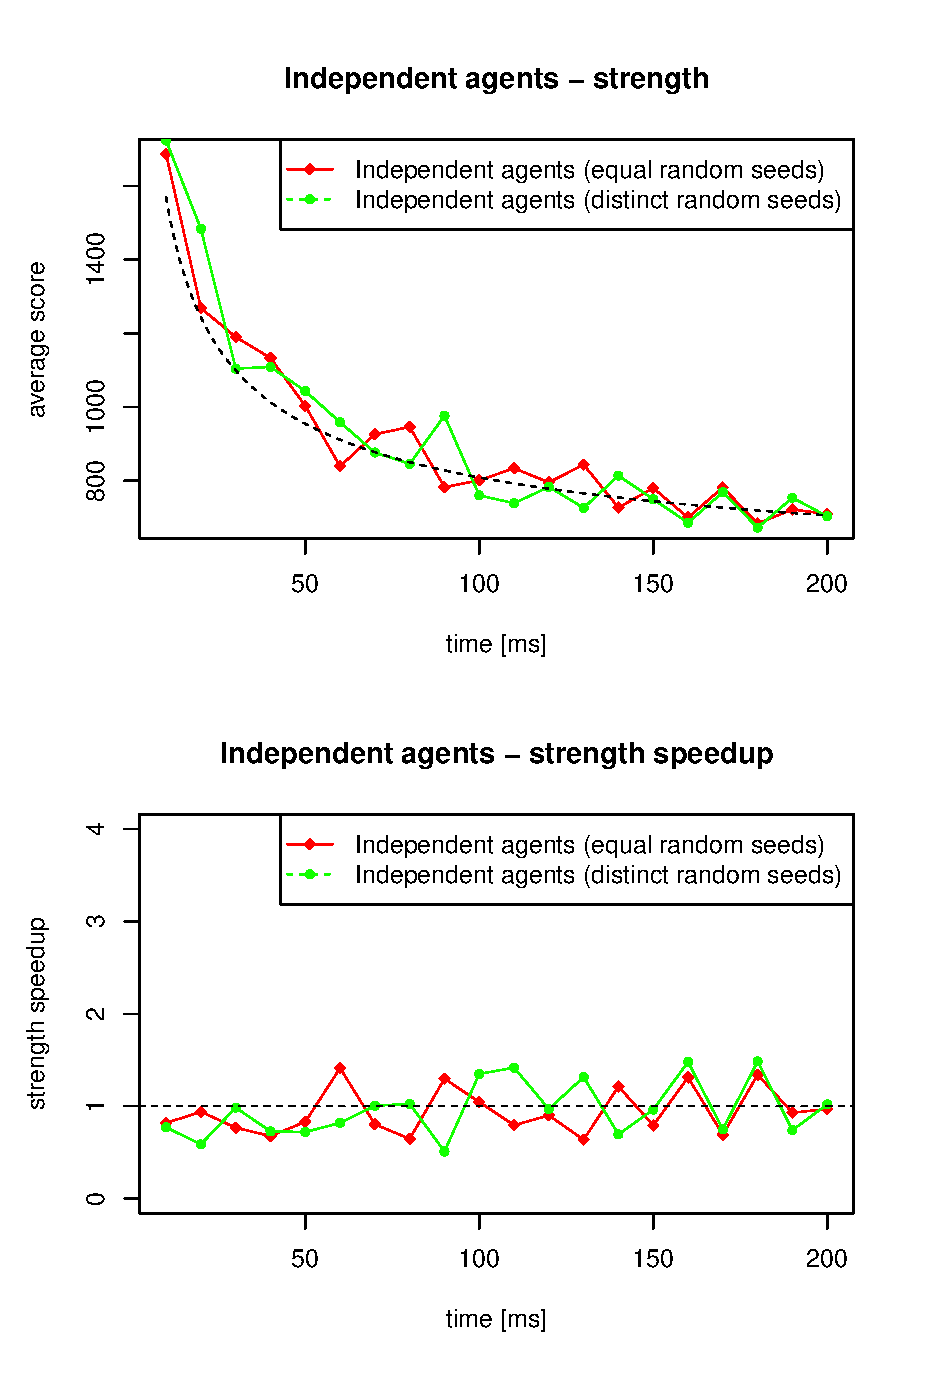
\includegraphics{img/dummy-ghosts-strength.eps}
\end{center}
\caption{\footnotesize Lorem ipsum}{\footnotesize }
\label{fig_independent_agents_strength}
\end{figure}

Independent agents does not perform any communication. Each of them build an independent MCTS
tree. The trees are synchronized by having same random seed for a construction of trees and so
trees are, after same number of interations, equal. For this algorithm, we expected strength
speedup approximately 1.0 or a bit lesser in case that the same-random-seed synchronization
doesn't always synchronize agents' actions.

For comparison, we tested also the independent agents algorithm with distinct random seeds.
Results are depicted by Figure \ref{fig_independent_agents_strength}. Average strength speedups
are 0.967 for equal random seeds and 0.941 for distinct random seeds what corresponds with
expectations.

Since there is no communication in algorithms, no further tests with altering communication
channel speed and channel reliability were done.


\todo{t-test na rozlišení významnosti rozdílu}


\subsection{Joint-Action Exchanging Agents}

\begin{figure}
\begin{center}
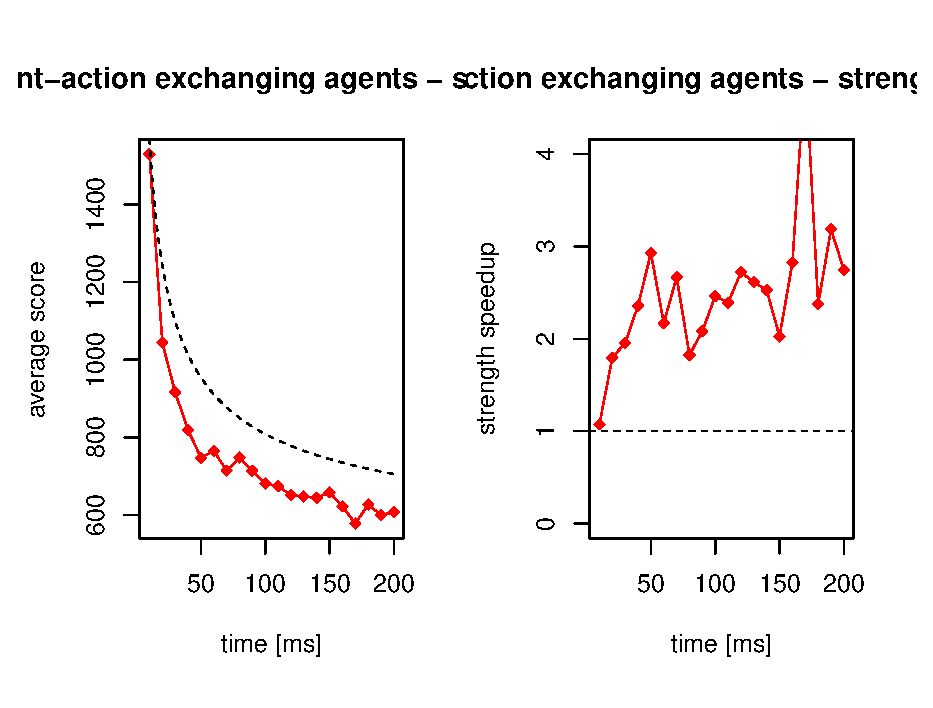
\includegraphics{img/move-exchange-strength.eps}
\end{center}
\caption{\footnotesize Lorem ipsum}{\footnotesize }
\label{fig_action_exchanging_strength}
\end{figure}

\todo{Doplnit avg strength-speedup}

Joint-action exchanging agents serves for comparing more complex coordination methods with the
simplest imaginable one. Particular agents use only simulations calculated by themselves and
the only way how the algorithm can outperform plain MCTS is by choosing the best of local
minima calculated by agents. However, accordingly to experiments, the algorithm performance was
at the level of plain MCTS and independent agents, with strength-speedup \emph{XXX}.
Performance of the algorithm ilustrates Figure \ref{fig_action_exchanging_strength}. Since
the joint-action exchange doesn't bring performance growth, measures with altering
communication channel settings were not performed.


\subsection{Root Exchanging Agents}

\begin{figure}
\begin{center}
\includegraphics{img/root-exchange-strength.eps}
\end{center}
\caption{\footnotesize Lorem ipsum}{\footnotesize }
\label{fig_root_exchanging_strength}
\end{figure}

\todo{Vše přepočítat, uvést počet simulací za sekundu,...}

Accordingly to good results of root parallelization algorithm referred in Section
\ref{sec_parallel_mcts_comparison}, we expected good behaviour of an algorithm based on this
parallelization. Root exchanging agents reached average strength speedup 2.48 (average strength
efficiency 0.62)) 
what is below our
expectation. Root parallelization tests performed on a domain of the game of Go
\cite{Chaslot2008} showed results of strength efficiency around 1. The difference may be caused
by different game played. In both root parallelization and root exchanging agents algorithm,
each thread/agent compute own tree doing the same exploration of an empty tree. In opposite,
plain MCTS does only one exploration and so remaining computational time is used for deeper
exploration. The exploration is probably more important for Ms Pac-Man game and so the
disadvantage of shallower exploitation shows itself by lesser strength efficiency. Expenses of
handling of messages in our implementation is below 0.2\% of total time so \todo{!}



\begin{figure}
\begin{center}
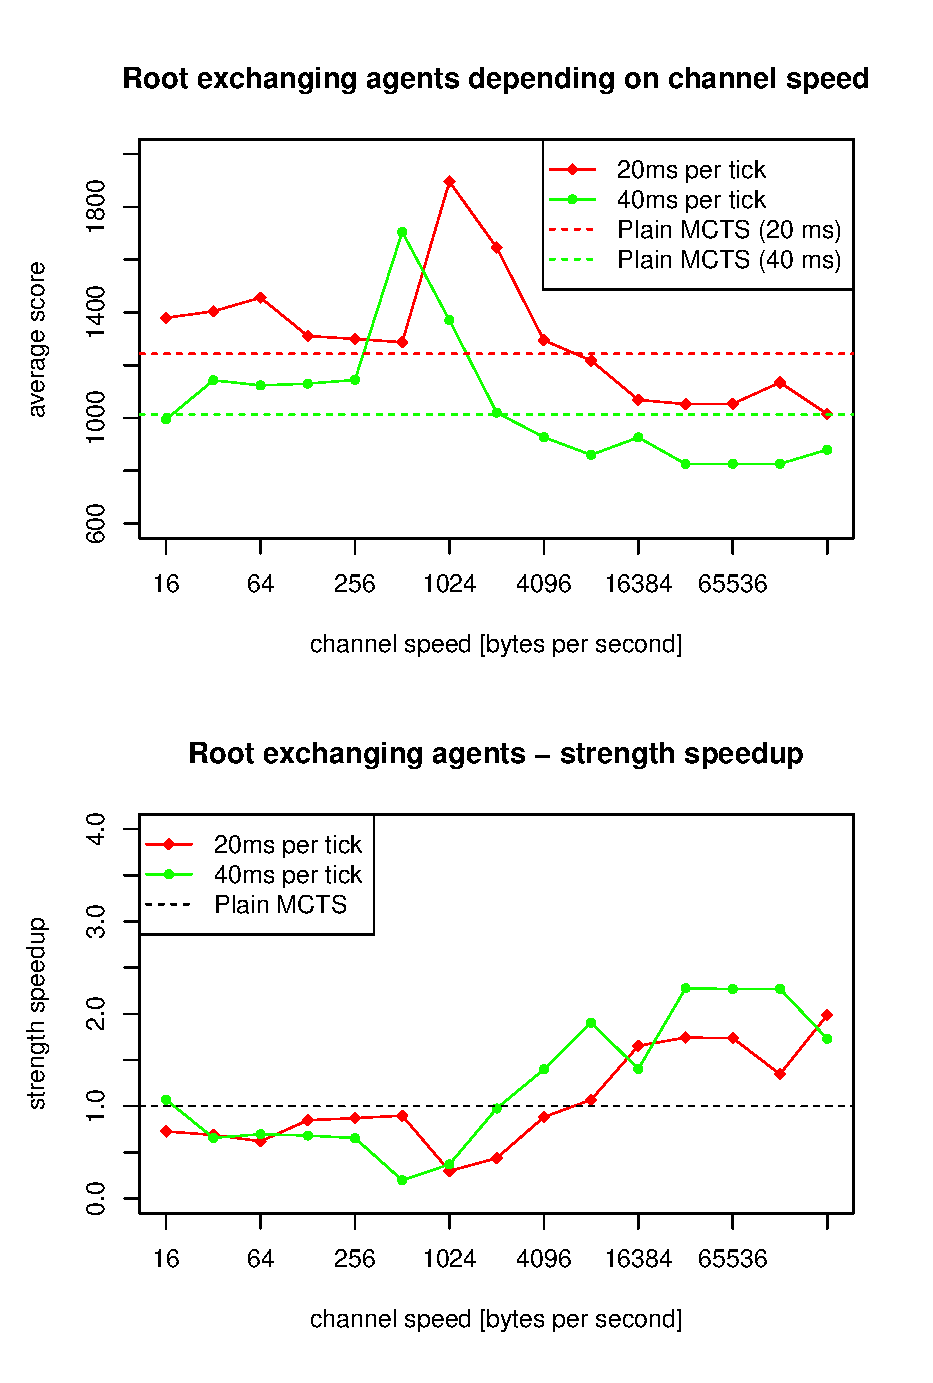
\includegraphics{img/root-exchange-channel-speed.eps}
\end{center}
\caption{\footnotesize Lorem ipsum}{\footnotesize }
\label{fig_root_exchanging_channel_speed}
\end{figure}




\subsection{Simulation Results Passing Agents}

\begin{figure}
\begin{center}
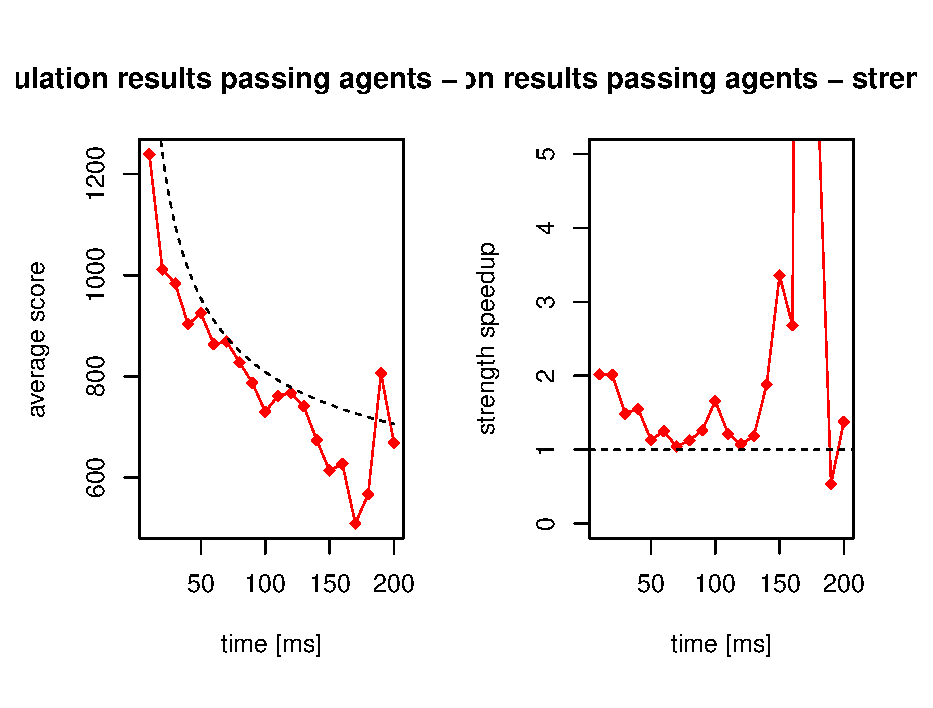
\includegraphics{img/simulation-passing-strength.eps}
\end{center}
\caption{\footnotesize Lorem ipsum}{\footnotesize }
\label{fig_simulation_passing_strength}
\end{figure}

\begin{figure}
\begin{center}
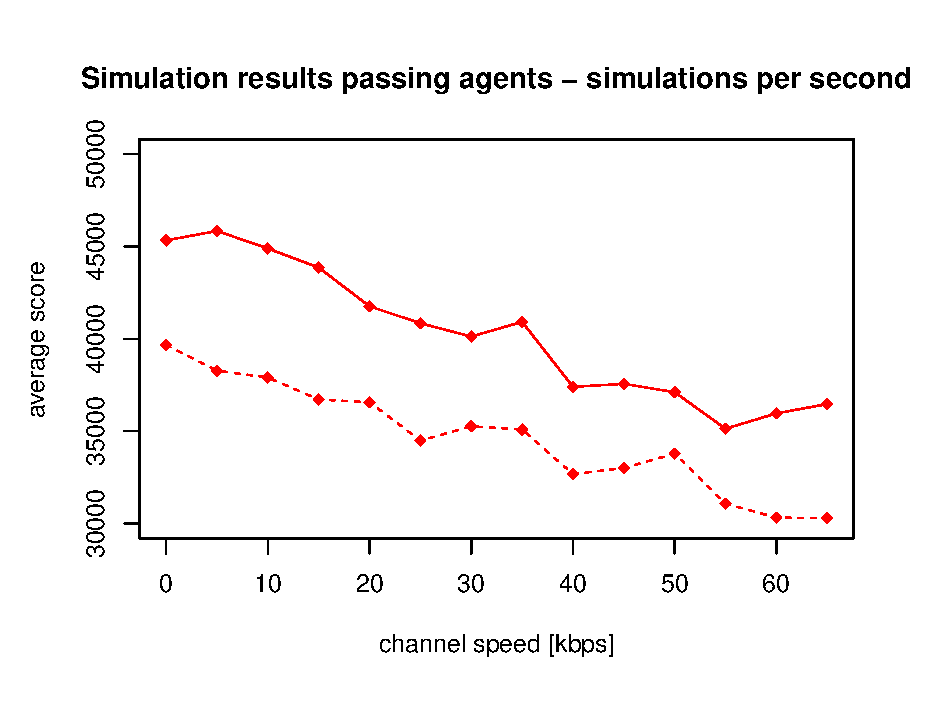
\includegraphics{img/simulation-passing-sims-per-sec.eps}
\end{center}
\caption{\footnotesize Lorem ipsum}{\footnotesize }
\label{fig_simulation_passing_sims_per_sec}
\end{figure}

\subsection{Tree-Cut Exchanging Agents}


\begin{figure}
\begin{center}
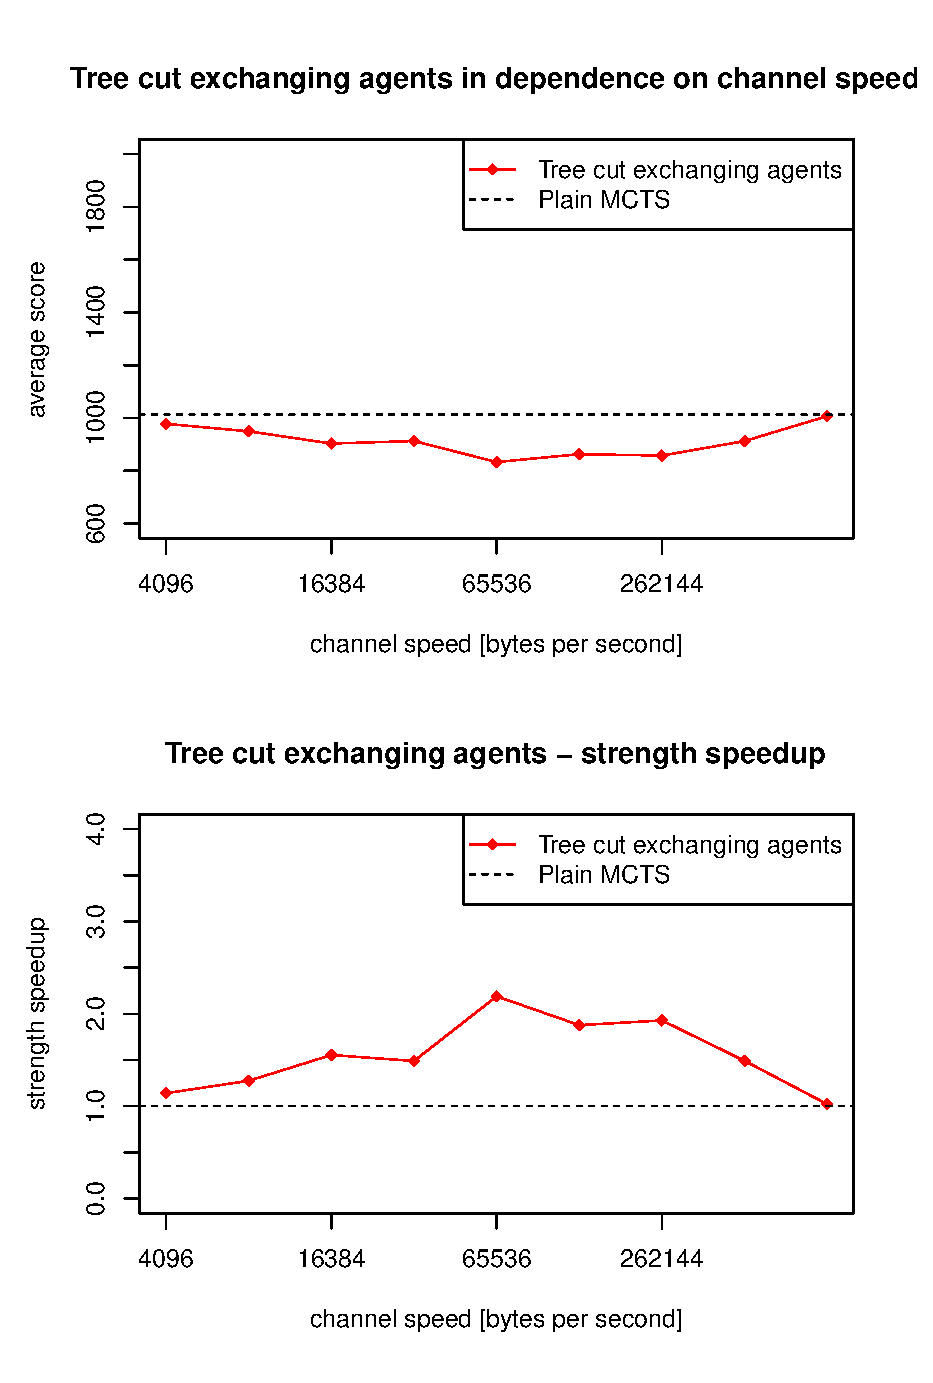
\includegraphics{img/tree-cut-channel-speed.eps}
\end{center}
\caption{\footnotesize Lorem ipsum}{\footnotesize }
\label{fig_tree_cut_channel_speed}
\end{figure}

\begin{figure}
\begin{center}
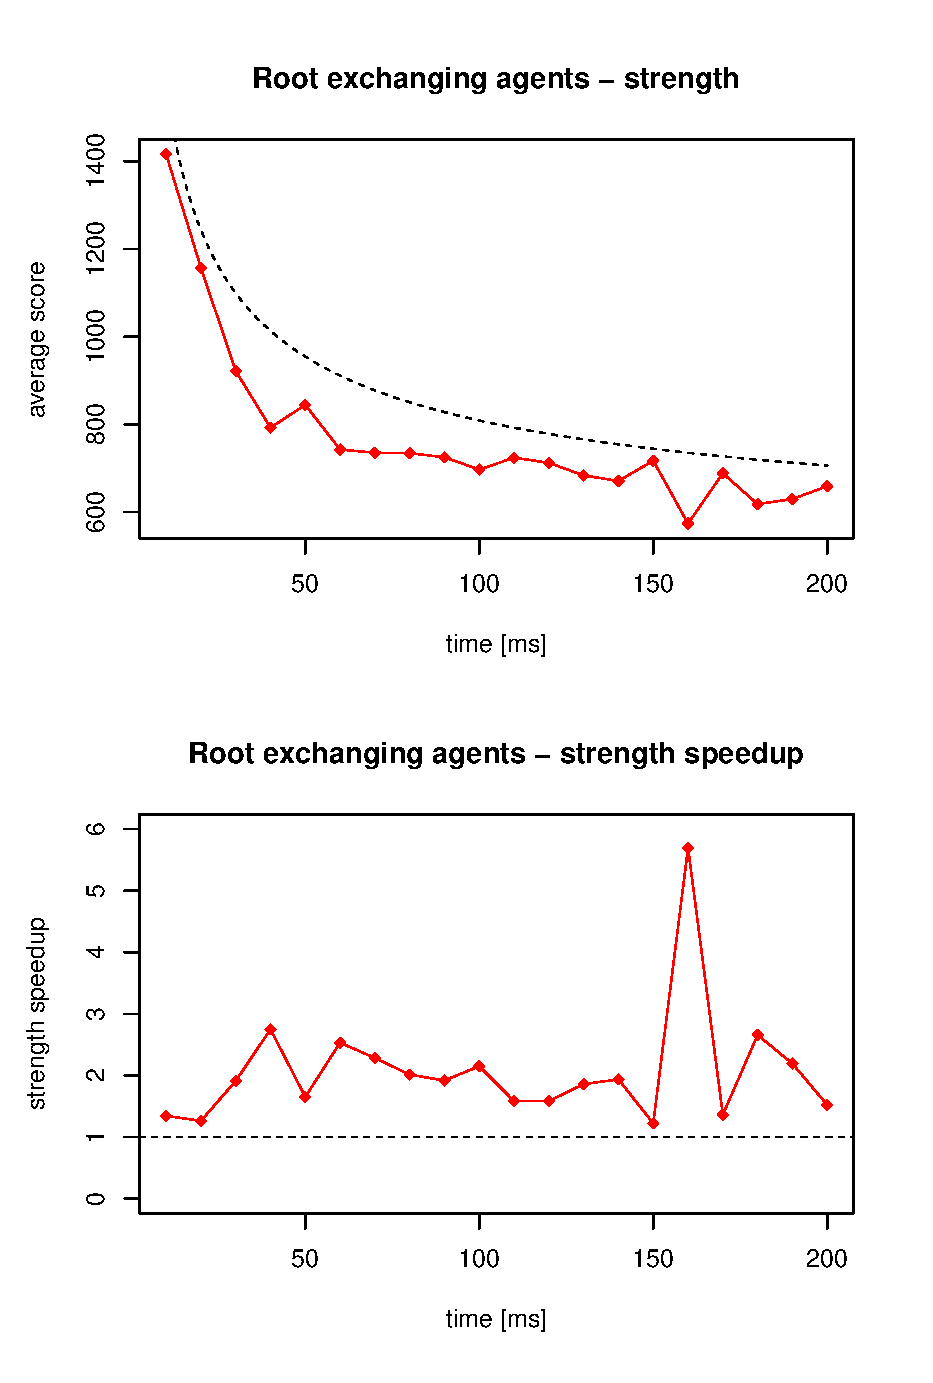
\includegraphics{img/tree-cut-strength.eps}
\end{center}
\caption{\footnotesize Lorem ipsum}{\footnotesize }
\label{fig_tree_cut_strength}
\end{figure}

\subsection{Comparison}

\section{Conclusion}
